\section{Motivation}
\subsection{The physics}

\begin{frame}{}{}
	\begin{columns}
	 	\column{.3\textwidth}
	 		\begin{center} 
				
\includegraphics[height=4cm]{penguino}
			\end{center}
	    \column{.65	\textwidth}
	    	\begin{block}{$K^+ \rightarrow \pi^+ \nu \bar{\nu} ~\Leftrightarrow ~
	    	V_{td}$ of CKM matrix} SM branching ratio: $(8.5\pm 0.7)\cdot 10^{-11}$ \\
	    	Strong impact by new physcis
			\end{block}
			\begin{block}{Measurement from BNL (Brookhaven)}
				The only experimental data so far (7 candidates)
	    		E787 and E949:\\
	    		$BR(K^+ \rightarrow \pi^+ \nu \bar{\nu})=(17.3^{+11.5}_{-10.5})\cdot
	    		10^{-11}$
			\end{block}
			\begin{exampleblock}{NA62 aims $\sigma < 10\%$ with 100 events}
	    		$\approx 10^{13} ~ K^+$ decays in 2014-15
			\end{exampleblock}
	\end{columns}
	\begin{block}{}
		Inspired by Mr. Heuer: Finding the needle in the \textbf{needlestack}
	\end{block}
\end{frame}


%\begin{frame}{What it does mean}{}
%	1 out of $10^{10}$ decays is like taking a 227~kB picture of every human
%	being on earth and filtering those with red hair, green-brown eyes, 3
%	birthmarks at the right cheek, age of\ldots until you have one person
%	remaining.
%	
%	\vspace{0.5cm}
%	\textbf{And we have to do that over 1000 times within two years!}
%	
%	\vspace{0.6cm}
%	\begin{center} 
%		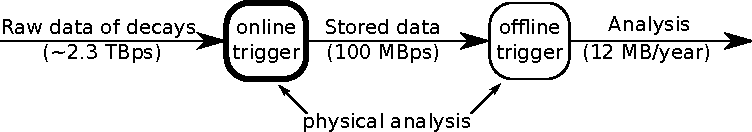
\includegraphics[width=\textwidth]{trigger-concept}
%	\end{center}
%
%\end{frame}


\section{The experiment}

%\begin{frame}{Background channels to be suppressed by the detector}{}
%	The main background channels to be separated from $K^+ \rightarrow \pi^+ \nu
%	\bar{\nu}$:
%	\begin{align*}
%	   K^+ &\rightarrow \mu^+ \nu &(63\%) &\rightarrow \mu \text{ veto} \\
%		 K^+ &\rightarrow \pi^+ \pi^0 &(21\%) &\rightarrow \gamma \text{ veto} \\
%	  	 K^+ &\rightarrow \pi^+ \pi^+ \pi^- &(6\%) &\rightarrow \text{charged
%	  	 % particle veto} \\
%	  	 K^+ &\rightarrow \pi^0 e^+ \nu &(5\%) &\rightarrow \gamma \text{ veto}  \\
%	  	  K^+ &\rightarrow \pi^0 \mu^+ \nu &(3\%) &\rightarrow \gamma, \mu \text{
%	  	  % veto} \\
%	  	   K^+ &\rightarrow \pi^+ \pi^0 \pi^0 &(2\%) &\rightarrow \gamma \text{
%	  	  veto}		  	
%	\end{align*}
%	\begin{ergo}
%		Detector dominated by vetos
%	\end{ergo}
%\end{frame}


\subsection{Subdetectors}
\begin{frame}{Experiment overview}{}
	\begin{columns}
	 	\column{.35\textwidth}
	 	\begin{block}{$K^+$ production}
	    		400 GeV protons from SPS colliding with a beryllium target
			\end{block}
	    \column{.6	\textwidth}
	    	\begin{block}{Measurement}
		    	\begin{itemize}
		    	  \item 0.8 GHz particles crossing\\ (6\% kaons)
				  \item 11 detectors triggered at 10 MHz
				\end{itemize}	    		
			\end{block}
	\end{columns}
	
	\begin{center} 
		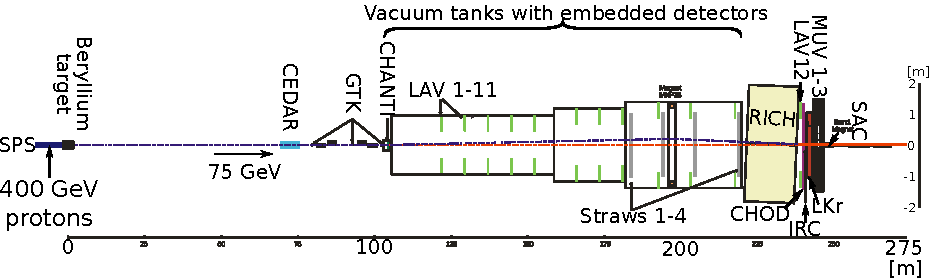
\includegraphics[width=\textwidth]{na62-overview-eng}
	\end{center}
\end{frame}

\begin{frame}{Data rates}{}
	\begin{center}
		\textbf{10 MHz unsteady $K^+$ decay rate}
	\end{center}
	\begin{table}[H]
		\begin{center}
			\begin{tabular}{c|c|>{\centering\arraybackslash}m{3cm}}
			Detector	&	Event size [B] &	Data rate [GBps]\\
			\hline
			CEDAR	&	216		&	2.16	\\
			GTK 	&	2250	&	22.50 	\\
			CHANTI	&	192		&	1.92 	\\
			LAV 	&	160		&	1.60 	\\
			STRAW 	&	768		&	7.68 	\\
			RICH 	&	160		&	1.60 	\\
			CHOD	&	$\ll1000$	&	$\ll10$\\
			MUV 	&	768		&	7.68 \\
			IRC \& SAC 	& 576	& 	5.76 	\\
			\textbf{LKR}		&	\textbf{222~k}	&	\textbf{2220}	\\
			\hline
			\textbf{Sum}	&	\textbf{$\approx$227~kB}	&	\textbf{$\approx$2.3~TBps}\\
			\end{tabular}
		\end{center}
	\end{table}
\end{frame}